\onehalfspacing
We simulated homogeneous sets of synthetic data for given stress tensors by generating slip on a series of randomly oriented fault planes. Then, we artificially mixed homogeneous sets to create a polyphase fault-slip data. Three types of tests are carried out, described as follows:

\section{Subsets with Similar Orientations}
We mixed two homogeneous synthetic data sets with same orientations of the principal stress axes, but different stress ellipsoid ratios (Table 4). The results of separation (Fig. 7A) show that GAPS is able to satisfactorily separate the polyphase data set with similar orientation of stresses, and only one fault in each phase is misclassified.

\section{Relatively Uneven Subsets}
In the second test, the polyphase data consists of slip generated on 5 faults from one stress tensor, and slip generated on 15 faults from a different stress tensor. The results, presented in Fig. 7B, show the efficacy of GAPS to separate the data having relatively uneven number of observations points in each phase.  Leisa and Lisle (2004) showed that some methods, such as the Multiple Inverse Method (Yamaji, 2000), fail to separate this type of data set.

\section{Separation of Homogeneous Fault-slip Data}
In the third test, we run the GAPS on a homogeneous data set with two prescribed phases of separation. The results clearly show that one of the phases of separation is minor, and has less than four data points (Fig. 7C). Since our inversion problem consists of four variables to be estimated, the phase with less than four fault slip data obviously gives meaningless inversion results. This phase should be ignored, and we conclude that only one phase is present in the fault-slip data. 

The reason that GAPS gives one phase with less than four data points is entirely related to the composite misfit, that we use for inversion. Since we are minimizing the sum of mean misfit for each phase of faulting, one of the following cases is possible when we overestimate the number of phases in the fault-slip data, which is a single phase in this example:

\renewcommand{\theenumi}{\roman{enumi}}
\begin{enumerate}
    \item The data is separated into the prescribed number of phases, with each phase having more than four data sets. In this case, the inversion of each phase will point towards the same stress tensor, and will tell us exactly how many different stress tensors are present.
    \item The data is separated into the prescribed number of phases, with some of the phases having less than four data sets. In this case, we ignore the phases with less than four data sets, and only consider the inversion results of the significant phases, that have more than four sets.
\end{enumerate}

After numerous trials, we find that the second case is almost always prevalent in the GAPS, and we can determine the number of phases of faulting in a single algorithm run. In order to get more reliable results, and not exclude any of the data, we can then run the algorithm a second time with known number of phases in the data.

\begin{figure}[H]
\begin{subfigure}{\textwidth}
    \centering
    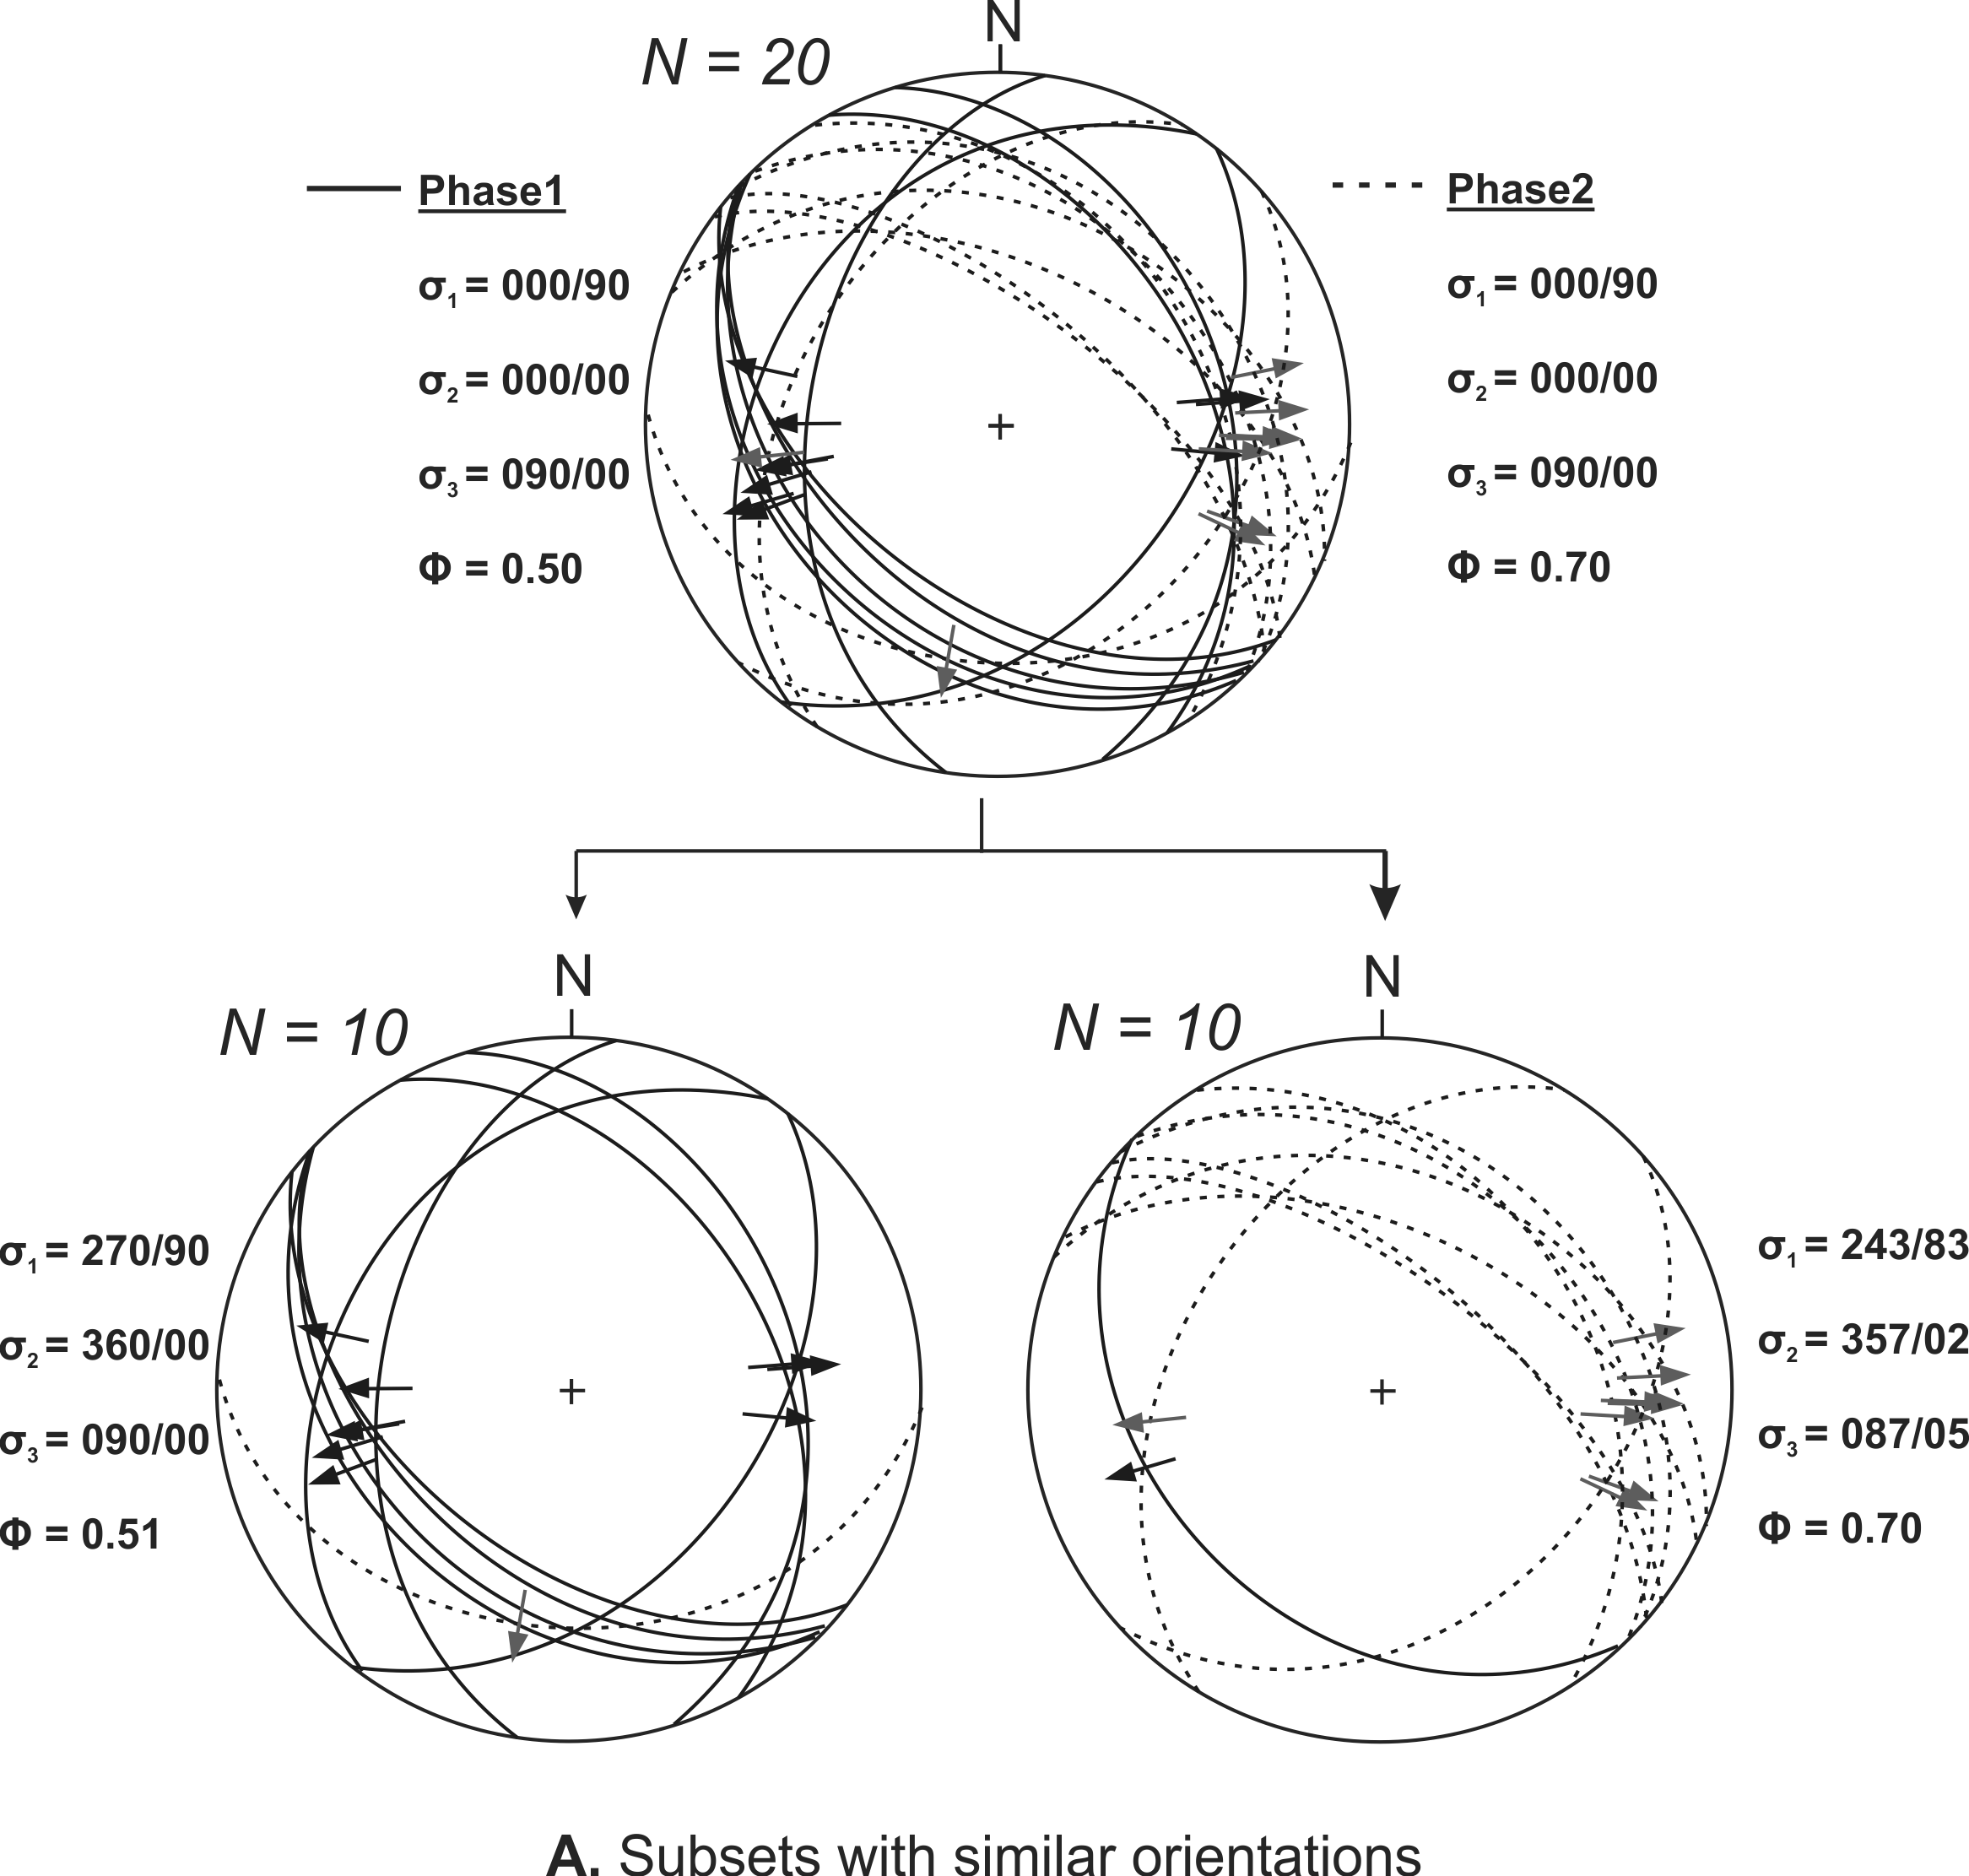
\includegraphics[scale = 0.6]{result2}
\end{subfigure}
\end{figure}
%\pagebreak
\begin{figure}[H]
\ContinuedFloat
\begin{subfigure}{\textwidth}
    \centering
    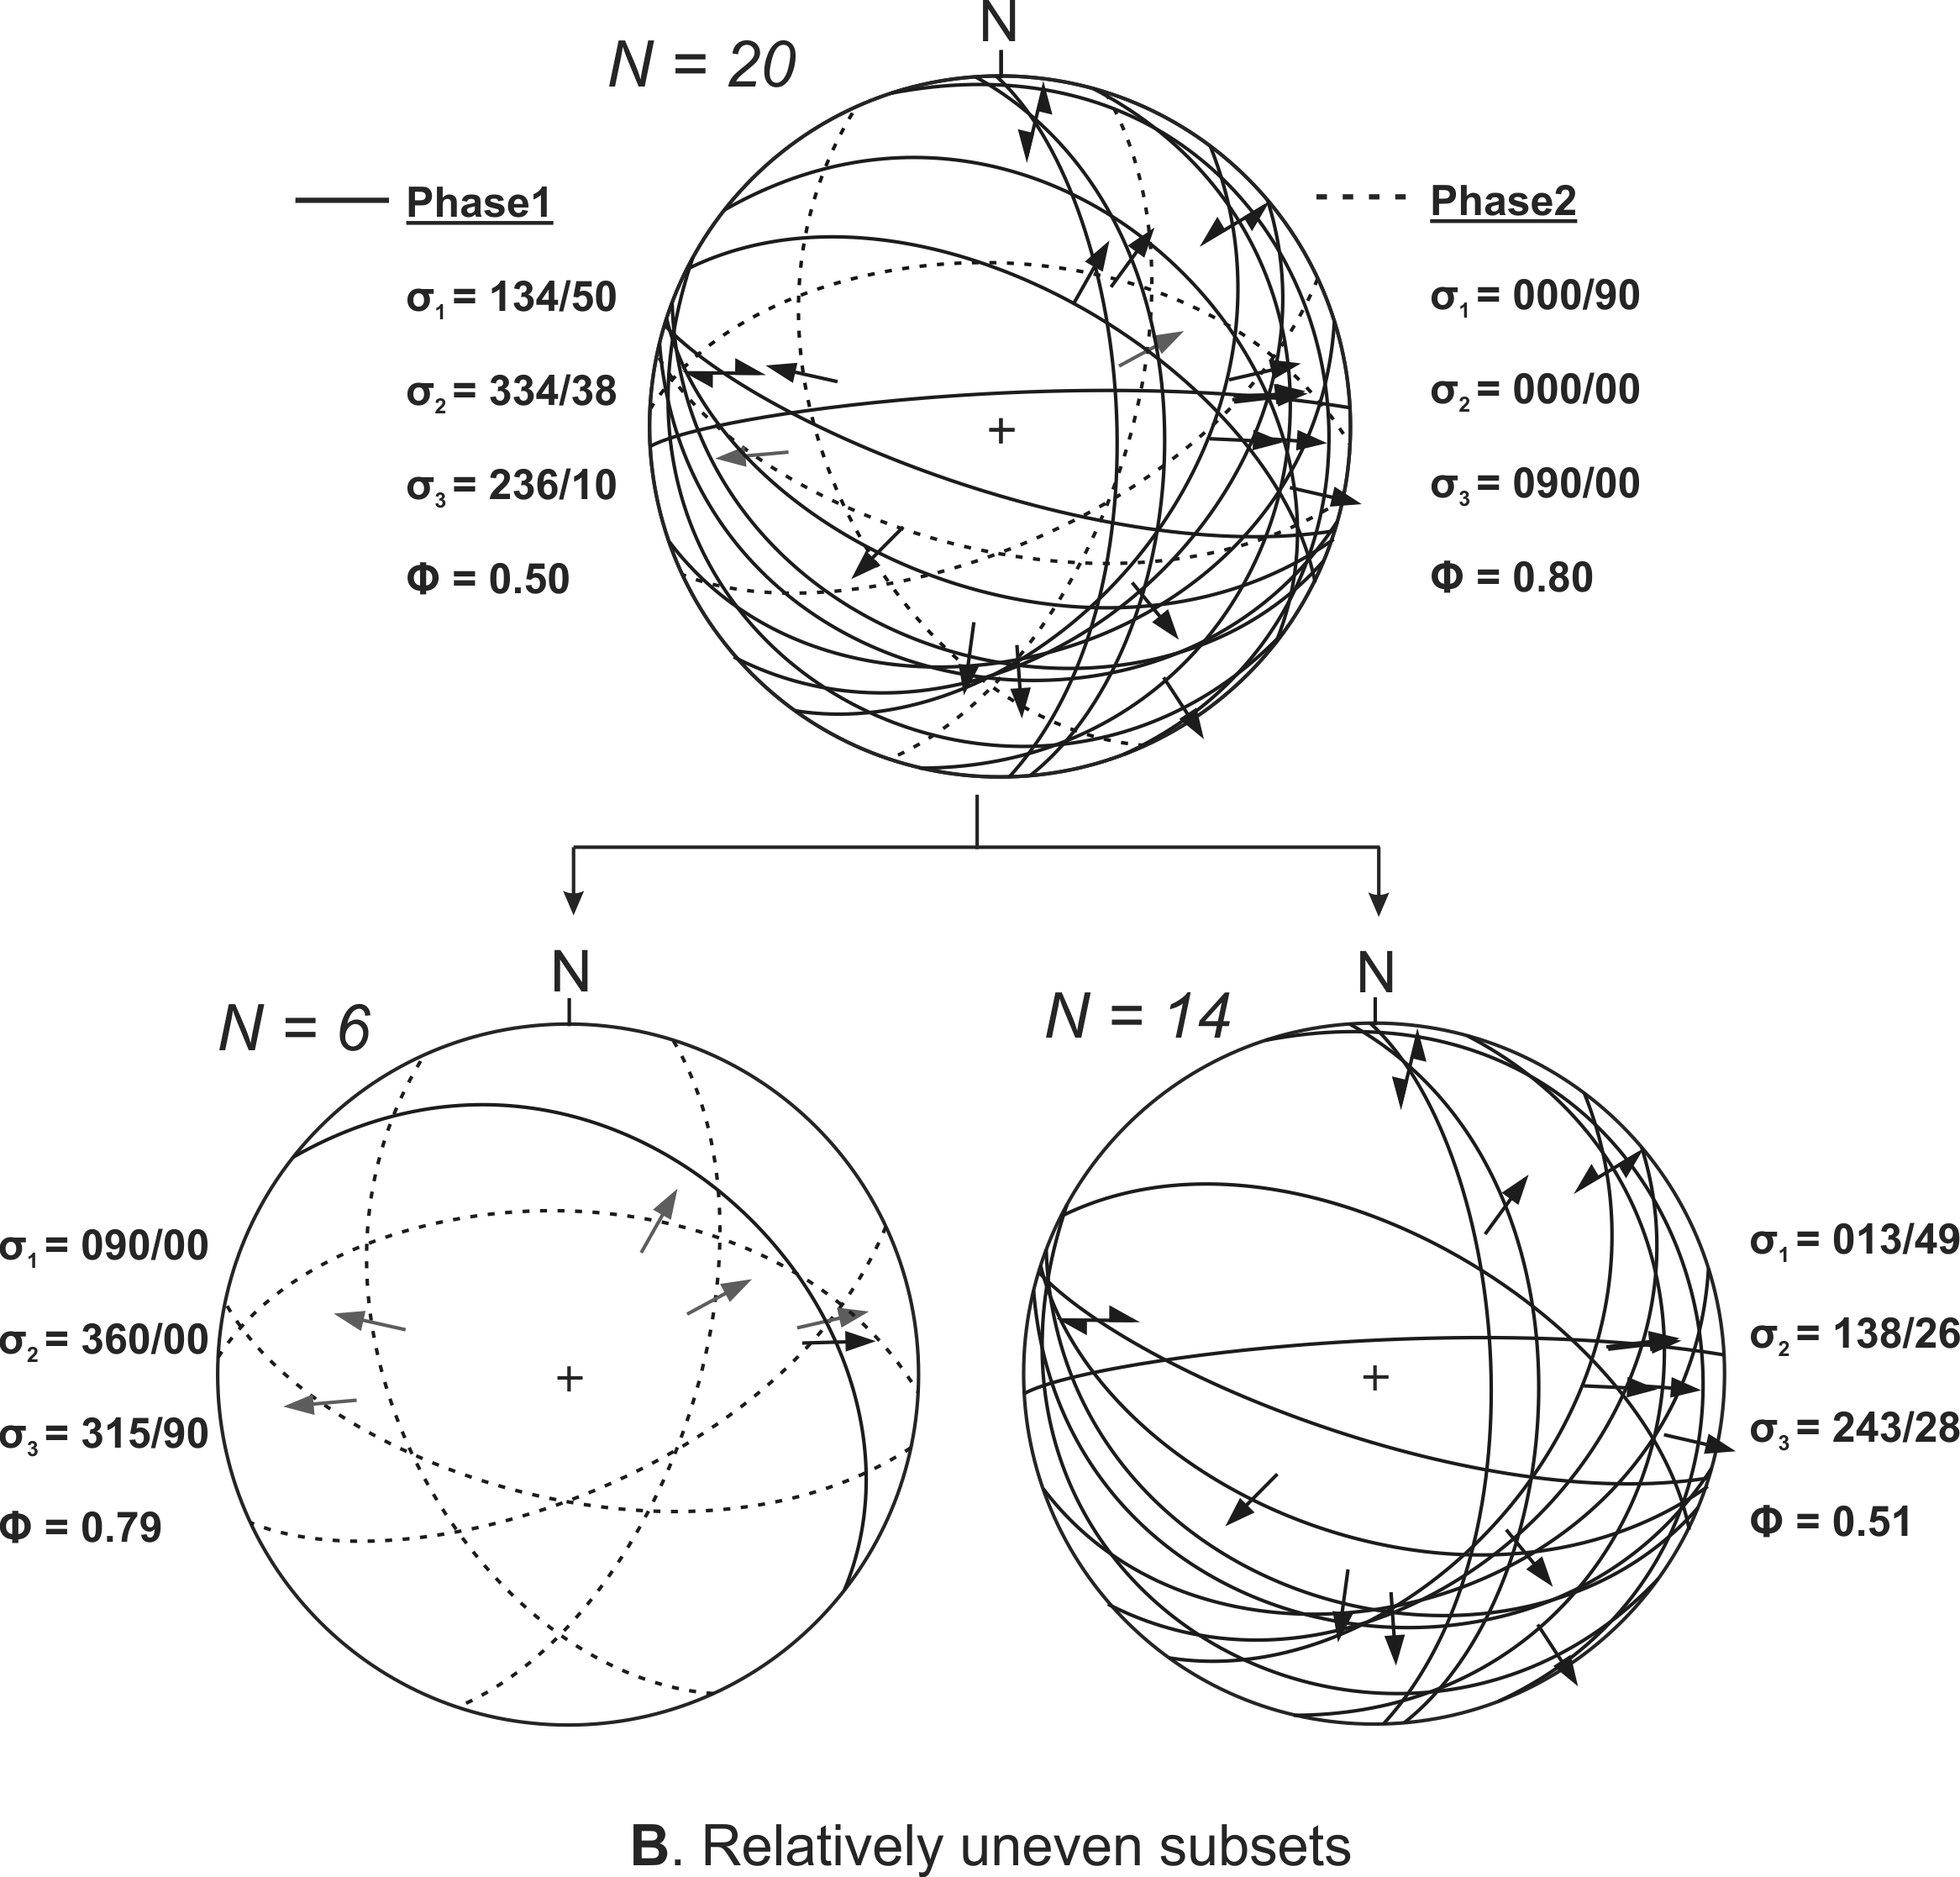
\includegraphics[scale = 0.6]{result2b}
\end{subfigure}
\end{figure}
\begin{figure}[H]
\ContinuedFloat
\begin{subfigure}{\textwidth}
    \centering
    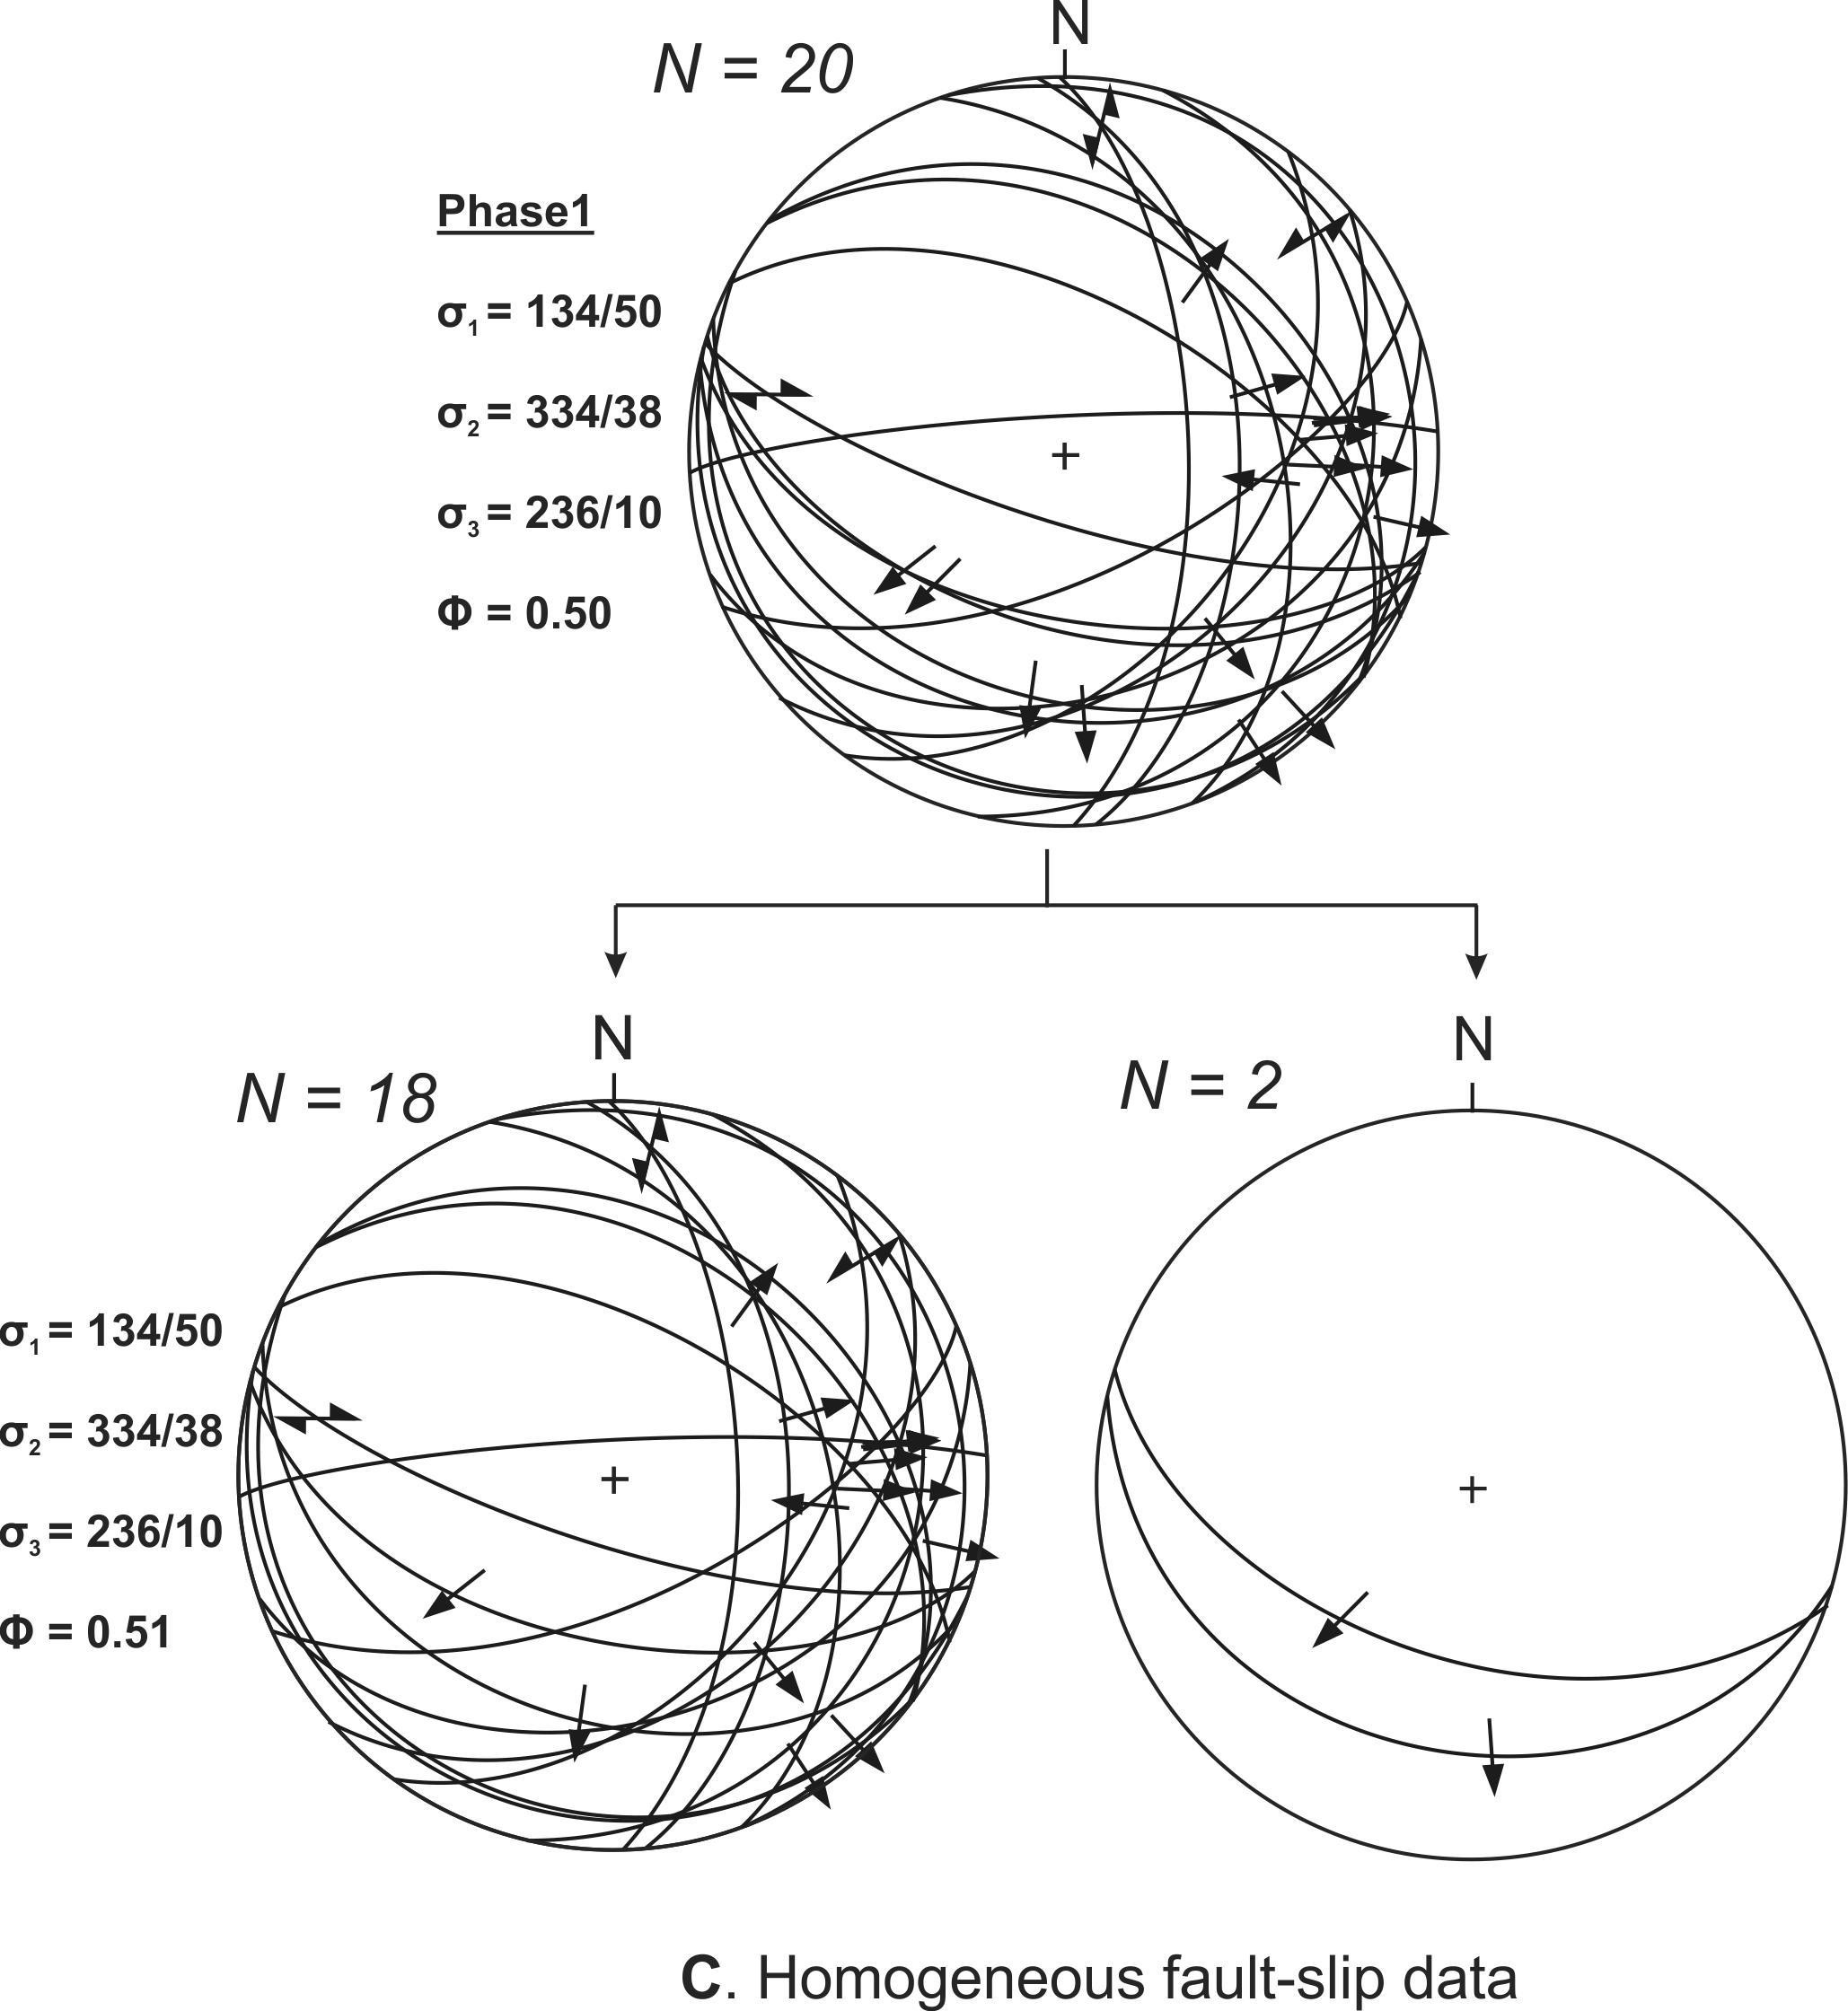
\includegraphics[scale = 0.6]{result2c}
\end{subfigure}
\caption{Separation of polyphase synthetic data sets. The top stereonet shows the synthetic mixed data set, and the bottom stereonets show the separation results.\textbf{A:} Subsets with similar orientation. \textbf{B:} Relatively uneven subsets. \textbf{C:} Separation of homogeneous fault-slip data. }
\end{figure}
